\documentclass[border=2pt]{standalone}
\usepackage{tikz}

% Brand colors (RGB normalized)
\definecolor{Garnet}{rgb}{0.451, 0.0, 0.039}
\definecolor{Atlantic}{rgb}{0.275, 0.416, 0.624}
\definecolor{Congaree}{rgb}{0.122, 0.255, 0.302}
\definecolor{Horseshoe}{rgb}{0.396, 0.471, 0.043}
\definecolor{Rose}{rgb}{0.8, 0.18, 0.251}
\definecolor{Honeycomb}{rgb}{0.643, 0.569, 0.216}
\definecolor{Grass}{rgb}{0.0, 0.8, 0.0}
\definecolor{Black90}{rgb}{0.212, 0.212, 0.212}
\definecolor{Black70}{rgb}{0.361, 0.361, 0.361}
\definecolor{Black50}{rgb}{0.635, 0.635, 0.635}
\definecolor{Black30}{rgb}{0.780, 0.780, 0.780}

\begin{document}
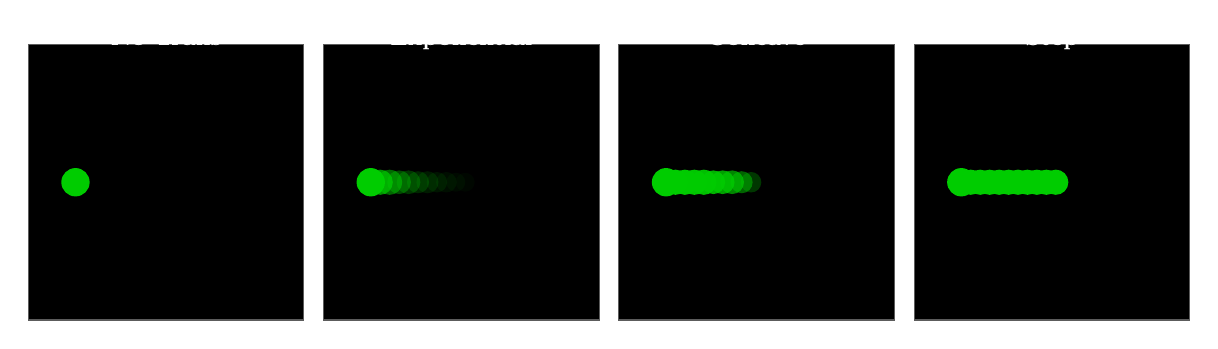
\begin{tikzpicture}[
  every node/.style={font=\footnotesize, inner sep=1pt}
]

% Panel dimensions
\def\pw{3.5}    % panel width cm
\def\ph{3.5}    % panel height cm
\def\gap{0.25}  % inter-panel gap cm

% Target position: center-left of each panel
% Target at (0.6, -1.75), trail extends to the right
\def\tx{0.6}    % target x within panel
\def\ty{-1.75}  % target y within panel
\def\tstep{0.12}% horizontal step between trail dots (overlapping for continuous streak)

% ============================================================
% PANEL 1: No Trails
% ============================================================
\def\ox{0}
\def\oy{0}

\fill[black] (\ox,\oy) rectangle (\ox+\pw, \oy-\ph);
\draw[Black70, line width=0.4pt] (\ox,\oy) rectangle (\ox+\pw, \oy-\ph);

% Single bright target dot only
\fill[Grass, opacity=1.0] (\ox+\tx, \oy+\ty) circle (0.18cm);

% Panel title
\node[white, font=\footnotesize\bfseries, anchor=north, align=center]
  at (\ox+\pw/2, \oy+0.22) {No Trails};

% ============================================================
% PANEL 2: Exponential decay  exp(-k/3)
% ============================================================
\def\ox{3.75}
\def\oy{0}

\fill[black] (\ox,\oy) rectangle (\ox+\pw, \oy-\ph);
\draw[Black70, line width=0.4pt] (\ox,\oy) rectangle (\ox+\pw, \oy-\ph);

% Trail dots: k=1..10, opacity = exp(-k/3)
% k=1: 0.716, k=2: 0.513, k=3: 0.368, k=4: 0.264, k=5: 0.189
% k=6: 0.135, k=7: 0.097, k=8: 0.069, k=9: 0.050, k=10: 0.036
\fill[Grass, opacity=0.716] (\ox+\tx+1*\tstep, \oy+\ty) circle (0.16cm);
\fill[Grass, opacity=0.513] (\ox+\tx+2*\tstep, \oy+\ty) circle (0.16cm);
\fill[Grass, opacity=0.368] (\ox+\tx+3*\tstep, \oy+\ty) circle (0.15cm);
\fill[Grass, opacity=0.264] (\ox+\tx+4*\tstep, \oy+\ty) circle (0.15cm);
\fill[Grass, opacity=0.189] (\ox+\tx+5*\tstep, \oy+\ty) circle (0.14cm);
\fill[Grass, opacity=0.135] (\ox+\tx+6*\tstep, \oy+\ty) circle (0.14cm);
\fill[Grass, opacity=0.097] (\ox+\tx+7*\tstep, \oy+\ty) circle (0.13cm);
\fill[Grass, opacity=0.069] (\ox+\tx+8*\tstep, \oy+\ty) circle (0.13cm);
\fill[Grass, opacity=0.050] (\ox+\tx+9*\tstep, \oy+\ty) circle (0.12cm);
\fill[Grass, opacity=0.036] (\ox+\tx+10*\tstep, \oy+\ty) circle (0.12cm);

% Target dot (current position, leftmost, brightest)
\fill[Grass, opacity=1.0] (\ox+\tx, \oy+\ty) circle (0.18cm);

% Panel title
\node[white, font=\footnotesize\bfseries, anchor=north, align=center]
  at (\ox+\pw/2, \oy+0.22) {Exponential};

% ============================================================
% PANEL 3: Concave decay  max(0, 1-(k/10)^3)
% ============================================================
\def\ox{7.50}
\def\oy{0}

\fill[black] (\ox,\oy) rectangle (\ox+\pw, \oy-\ph);
\draw[Black70, line width=0.4pt] (\ox,\oy) rectangle (\ox+\pw, \oy-\ph);

% k=1: 1-(0.1)^3=0.999, k=2: 1-(0.2)^3=0.992, k=3: 1-(0.3)^3=0.973
% k=4: 1-(0.4)^3=0.936, k=5: 1-(0.5)^3=0.875, k=6: 1-(0.6)^3=0.784
% k=7: 1-(0.7)^3=0.657, k=8: 1-(0.8)^3=0.488, k=9: 1-(0.9)^3=0.271
% k=10: 1-(1.0)^3=0.0
\fill[Grass, opacity=0.999] (\ox+\tx+1*\tstep, \oy+\ty) circle (0.16cm);
\fill[Grass, opacity=0.992] (\ox+\tx+2*\tstep, \oy+\ty) circle (0.16cm);
\fill[Grass, opacity=0.973] (\ox+\tx+3*\tstep, \oy+\ty) circle (0.16cm);
\fill[Grass, opacity=0.936] (\ox+\tx+4*\tstep, \oy+\ty) circle (0.16cm);
\fill[Grass, opacity=0.875] (\ox+\tx+5*\tstep, \oy+\ty) circle (0.15cm);
\fill[Grass, opacity=0.784] (\ox+\tx+6*\tstep, \oy+\ty) circle (0.15cm);
\fill[Grass, opacity=0.657] (\ox+\tx+7*\tstep, \oy+\ty) circle (0.15cm);
\fill[Grass, opacity=0.488] (\ox+\tx+8*\tstep, \oy+\ty) circle (0.14cm);
\fill[Grass, opacity=0.271] (\ox+\tx+9*\tstep, \oy+\ty) circle (0.13cm);
% k=10 opacity=0, omit

% Target dot
\fill[Grass, opacity=1.0] (\ox+\tx, \oy+\ty) circle (0.18cm);

% Panel title
\node[white, font=\footnotesize\bfseries, anchor=north, align=center]
  at (\ox+\pw/2, \oy+0.22) {Concave};

% ============================================================
% PANEL 4: Step decay (uniform full opacity, abrupt end)
% ============================================================
\def\ox{11.25}
\def\oy{0}

\fill[black] (\ox,\oy) rectangle (\ox+\pw, \oy-\ph);
\draw[Black70, line width=0.4pt] (\ox,\oy) rectangle (\ox+\pw, \oy-\ph);

% All trail dots at full opacity
\foreach \k in {1, 2, 3, 4, 5, 6, 7, 8, 9, 10}{
  \fill[Grass, opacity=1.0] (\ox+\tx+\k*\tstep, \oy+\ty) circle (0.16cm);
}

% Target dot
\fill[Grass, opacity=1.0] (\ox+\tx, \oy+\ty) circle (0.18cm);

% Panel title
\node[white, font=\footnotesize\bfseries, anchor=north, align=center]
  at (\ox+\pw/2, \oy+0.22) {Step};

\end{tikzpicture}
\end{document}
